\chapter{Analisi dei requisiti}
\label{cap:analisi-requisiti}

\intro{In questo capitolo verranno illustrati e descritti i casi d'uso del sistema applicativo e classificati i requisiti analizzati.}\\

\section{Casi d'uso}
\label{sec:usecase}

Per lo studio dei \gls{usecase}\glsoccur del prodotto sono stati creati degli appositi diagrammi che illustrano le interazioni tra gli attori e il sistema.\\
Ciascun caso d'uso viene fornito con una descrizione che ne riporta le informazioni principali, come attori coinvolti, pre e post condizioni, scenario principale ed eventuali scenari secondari.\\
Per questioni di leggibilità, i diagrammi sono stati suddivisi in più parti, raggrupando i casi d'uso che costituiscono una macro-funzionalità (?) del sistema.

\subsection{Attori}
\label{subsec:attori}

In questa sezione vengono definiti gli attori che interagiscono con il sistema.

\subsubsection{Attori primari}
\label{subsubsec:attori-primari}

\begin{itemize}
    \item \textbf{Utente non autenticato}: utente che possiede le credenziali per accedere al sistema, ma non ha ancora effettuato l'autenticazione;
    \item \textbf{Utente autenticato}: utente che ha effettuato l'autenticazione al sistema.
\end{itemize}

\subsubsection{Attori secondari}
\label{subsubsec:attori-secondari}

\begin{itemize}
    \item \textbf{\emph{RiskAPP API}}: sistema che fornisce le \gls{apig}\glsoccur del \emph{Tool Trattative} per l'interazione con il \gls{backend}\glsoccur dell'applicazione.
\end{itemize}

\clearpage

\begin{figure}[!h] 
    \centering 
    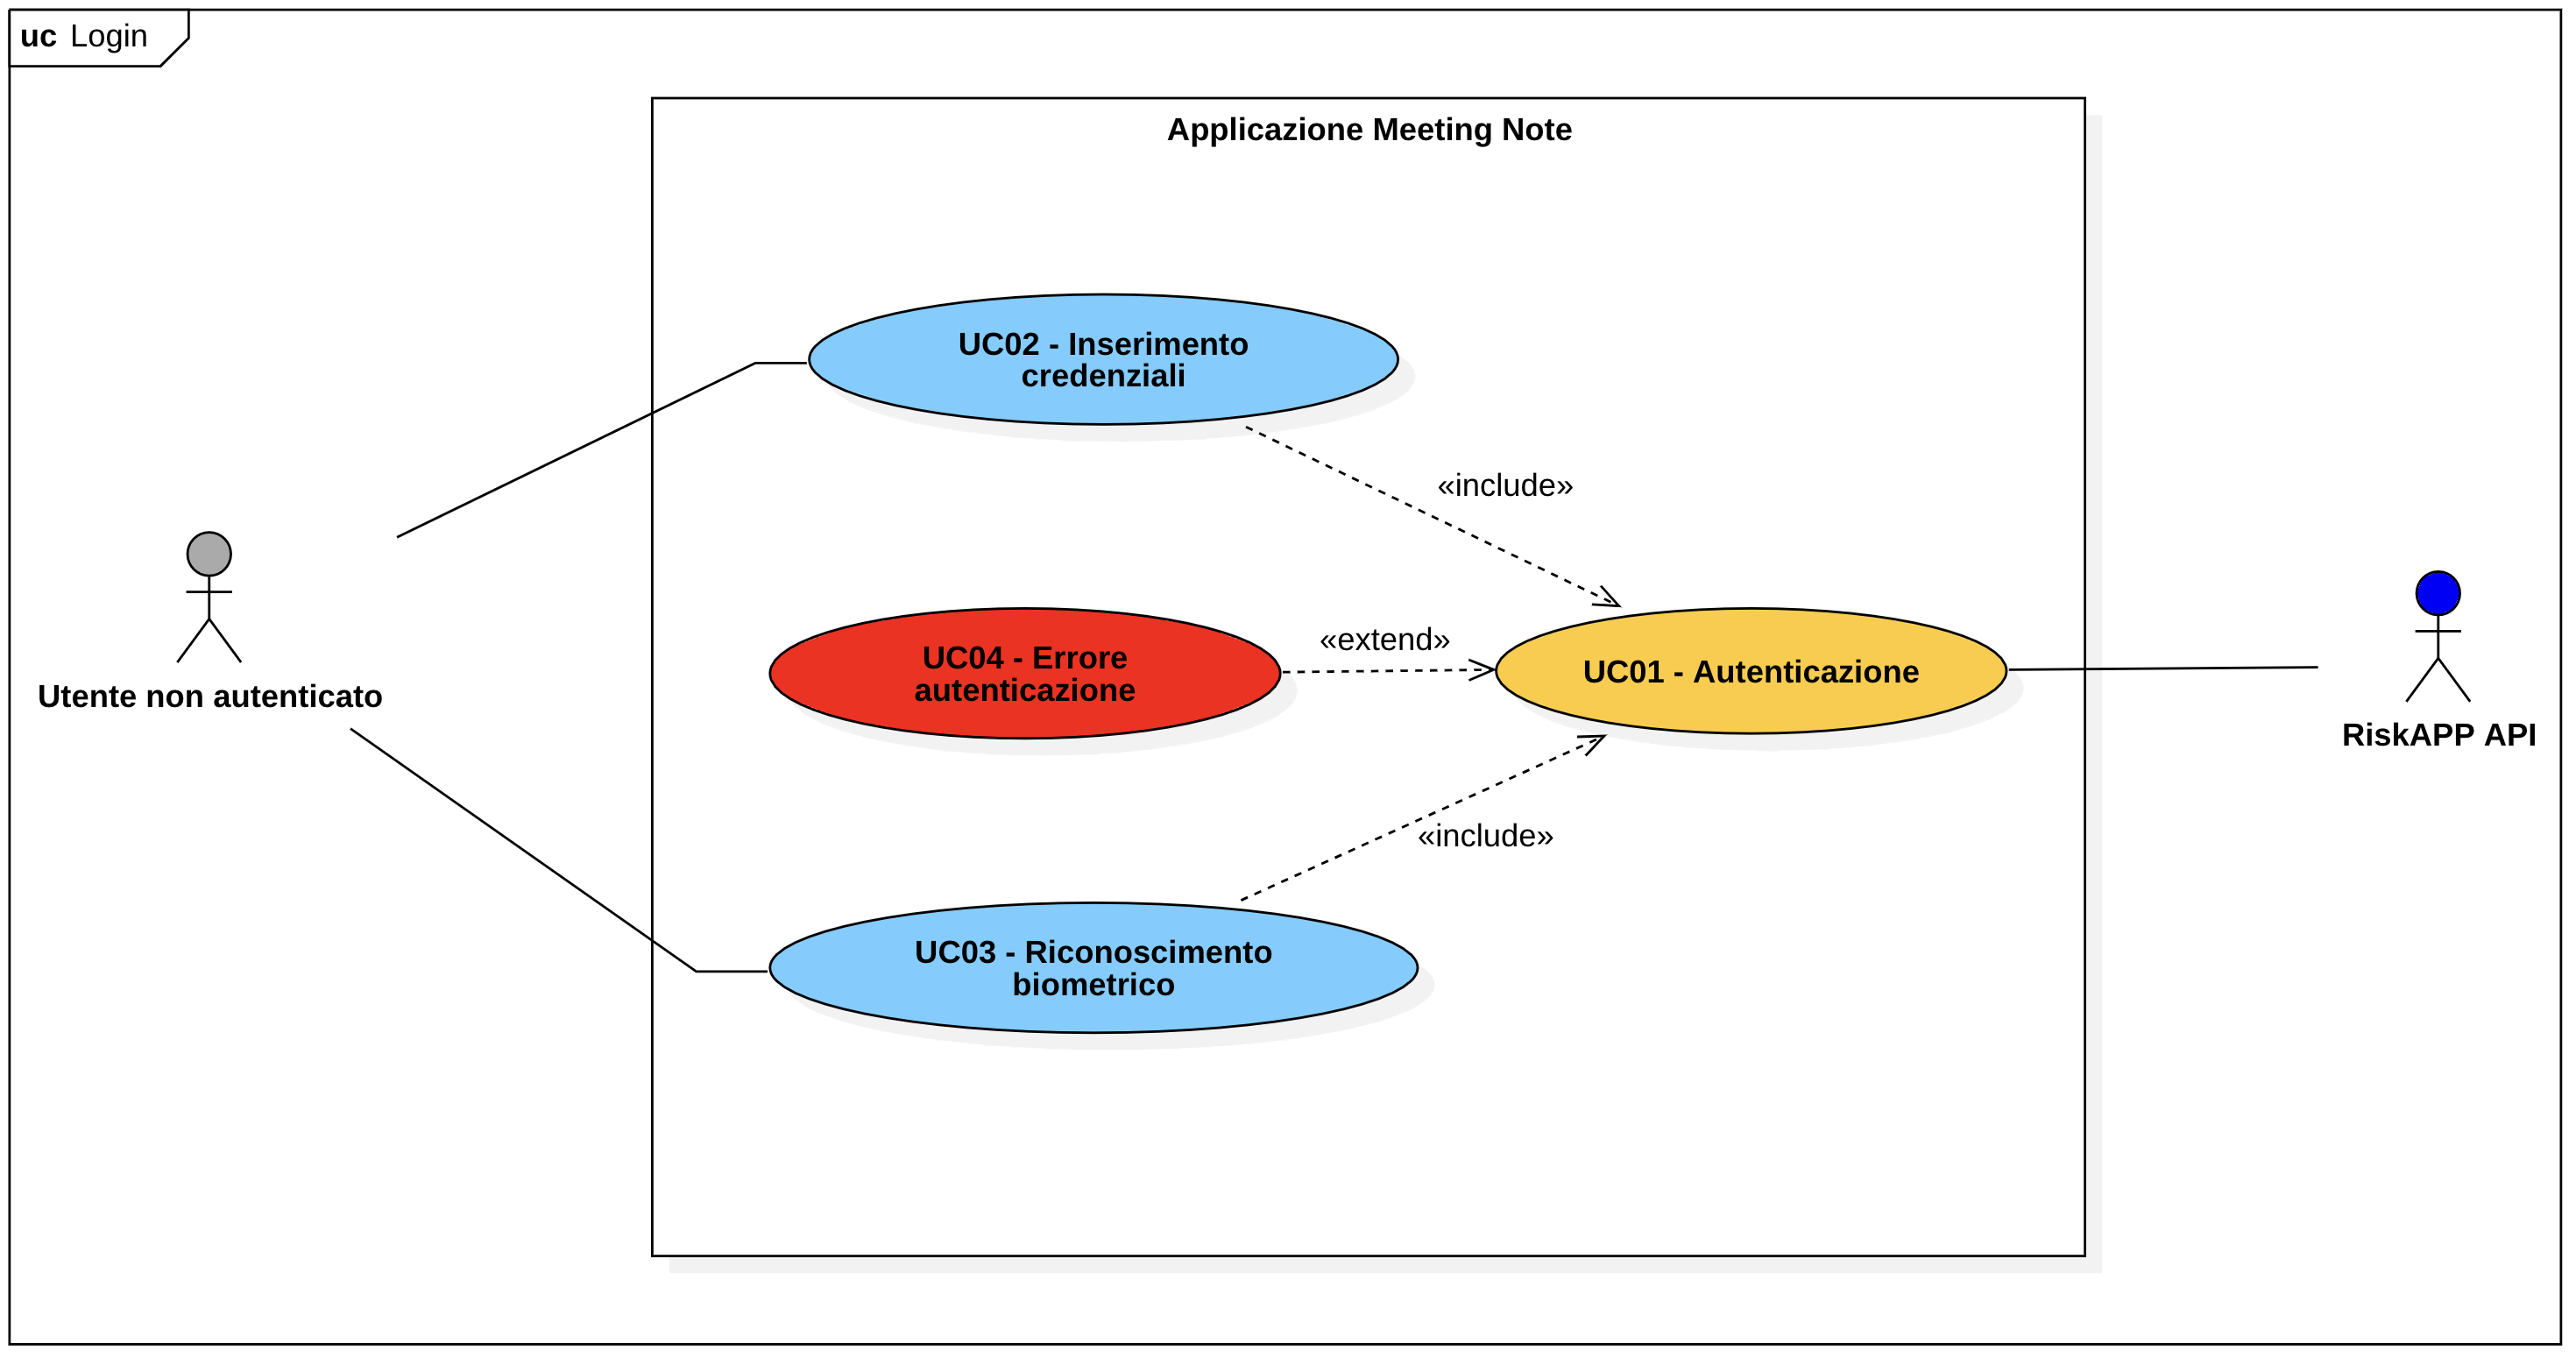
\includegraphics[width=1.0\columnwidth]{usecase/1-uc} 
    \caption{Use Case - Login}
\end{figure}

\begin{usecase}{01}{Autenticazione}
    \usecasemainactors{Utente non autenticato}
    \usecasesecondaryactors{\emph{RiskAPP API}}
    \usecasepre{L'utente non è ancora autenticato nel sistema}
    \usecasedesc{L'utente effettua l'autenticazione al sistema, scegliendo se farlo, inserendo manualmente le credenziali, oppure tramite \gls{riconoscimentobiometrico}\glsoccur.}
    \usecasepost{L'utente è autenticato nel sistema}
    \usecasealt{Se l'autenticazione fallisce, si verifica \hyperref[UC04]{UC04}}
    \label{UC01}
\end{usecase}

\begin{usecase}{02}{Inserimento credenziali}
    \usecasemainactors{Utente non autenticato}
    \usecasesecondaryactors{\emph{RiskAPP API}}
    \usecasepre{L'utente non è ancora autenticato nel sistema}
    \usecasedesc{L'utente inserisce manualmente le proprie credenziali per effettuare l'autenticazione al sistema.}
    \usecasepost{L'utente è autenticato nel sistema}
    \label{UC02}
\end{usecase}

\begin{usecase}{03}{Riconoscimento biometrico}
    \usecasemainactors{Utente non autenticato}
    \usecasesecondaryactors{\emph{RiskAPP API}}
    \usecasepre{L'utente non è ancora autenticato nel sistema}
    \usecasedesc{L'utente effettua il \gls{riconoscimentobiometrico}\glsoccur per effettuare l'autenticazione al sistema.}
    \usecasepost{L'utente è autenticato nel sistema}
    \label{UC03}
\end{usecase}

\begin{usecase}{04}{Errore autenticazione}
    \usecasemainactors{Utente non autenticato}
    \usecasepre{L'utente non è ancora autenticato nel sistema}
    \usecasedesc{L'autenticazione fallisce e l'utente viene informato dell'errore; le motivazioni possono essere le seguenti:
        \begin{itemize}
            \item le credenziali inserite non sono corrette;
            \item il sistema non è raggiungibile;
            \item connessione ad internet assente.
        \end{itemize}}
    \usecasepost{L'utente non è autenticato nel sistema}
    \label{UC04}
\end{usecase}

\begin{figure}[!h] 
    \centering 
    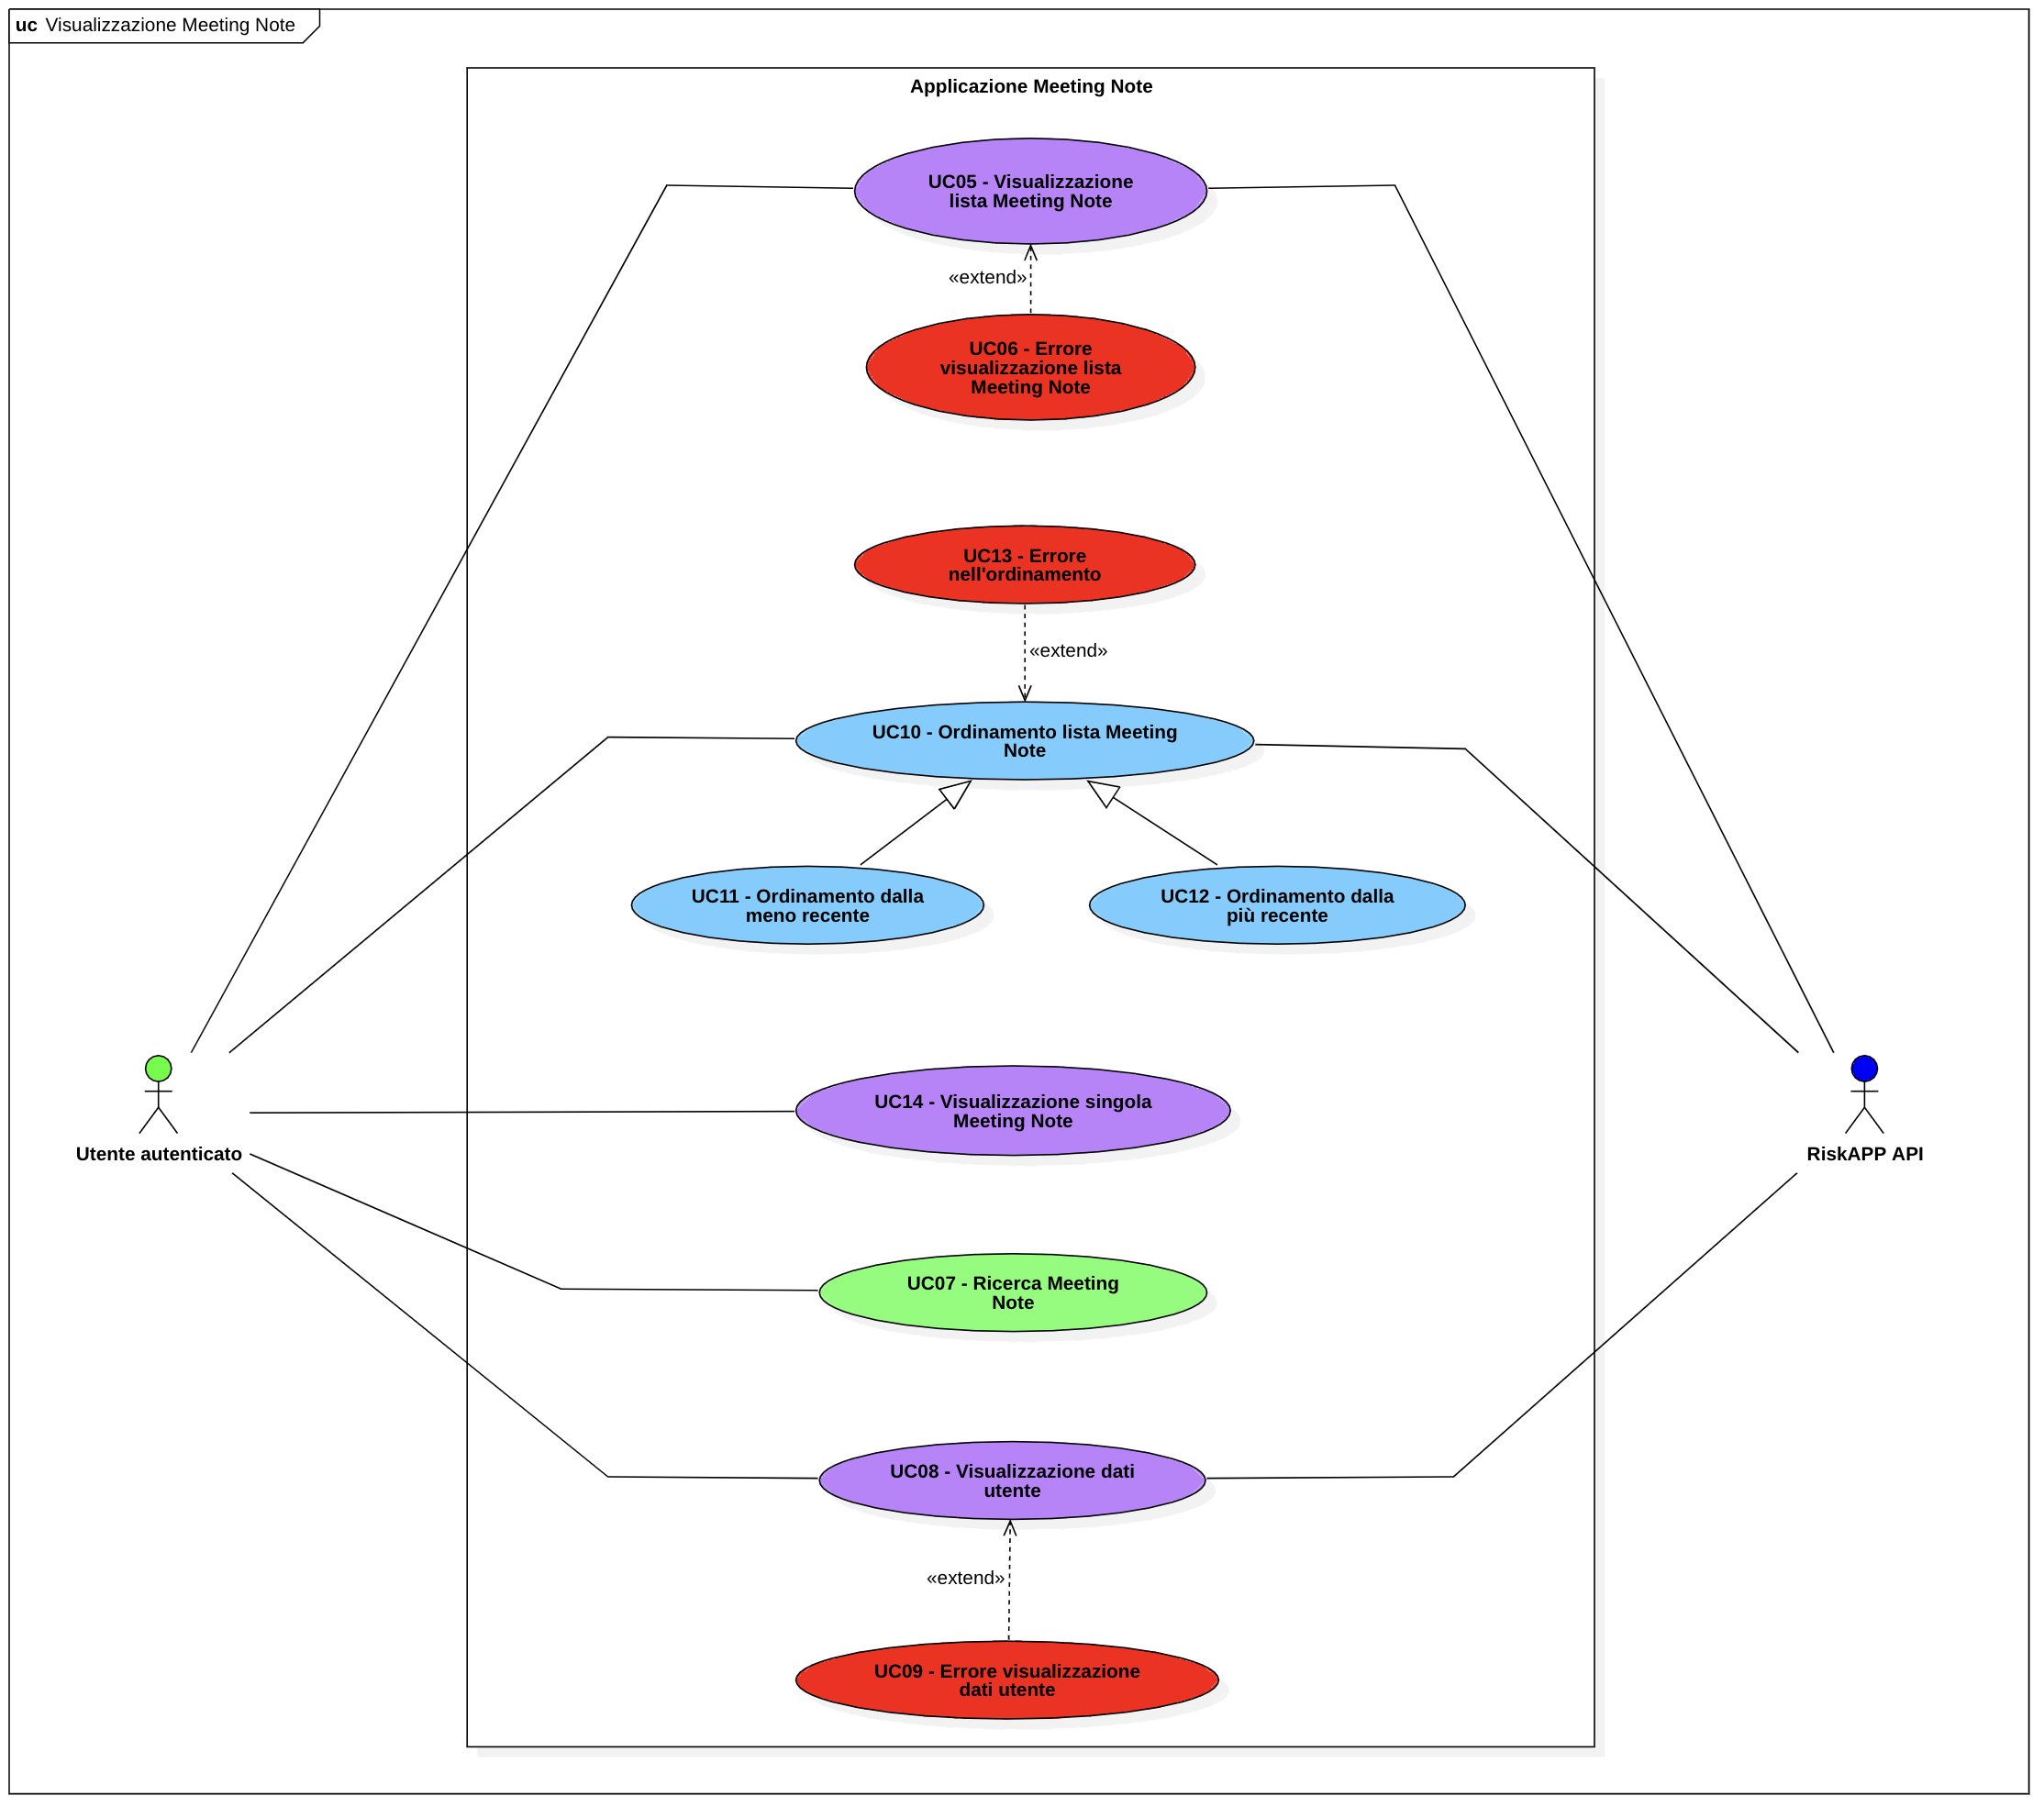
\includegraphics[width=1.0\columnwidth]{usecase/2-uc} 
    \caption{Use Case - Visualizzazione Meeting Note}
\end{figure}

\begin{usecase}{05}{Visualizzazione Meeting Note}
    \usecasemainactors{Utente autenticato}
    \usecasesecondaryactors{\emph{RiskAPP API}}
    \usecasepre{L'utente è autenticato nel sistema}
    \usecasedesc{Viene visualizzata la lista di tutte le \gls{meetingnote}\glsoccur associate all'utente autenticato.}
    \usecasepost{L'utente visualizza la lista delle \gls{meetingnote}\glsoccur}
    \usecasealt{Se la visualizzazione fallisce, si verifica \hyperref[UC06]{UC06}}
    \label{UC05}
\end{usecase}

\begin{usecase}{06}{Errore visualizzazione lista Meeting Note}
    \usecasemainactors{Utente autenticato}
    \usecasepre{L'utente è autenticato nel sistema}
    \usecasedesc{La visualizzazione della lista delle \gls{meetingnote}\glsoccur fallisce e l'utente viene informato dell'errore; le motivazioni possono essere le seguenti:
        \begin{itemize}
            \item la lista è vuota;
            \item il sistema non è raggiungibile;
            \item token di autenticazione scaduto;
            \item connessione ad internet assente.
        \end{itemize}}
    \usecasepost{L'utente non visualizza la lista delle \gls{meetingnote}\glsoccur}
    \label{UC06}
\end{usecase}

\section{Tracciamento dei requisiti}

Da un'attenta analisi dei requisiti e degli use case effettuata sul progetto è stata stilata la tabella che traccia i requisiti in rapporto agli use case.\\
Sono stati individuati diversi tipi di requisiti e si è quindi fatto utilizzo di un codice identificativo per distinguerli.\\
Il codice dei requisiti è così strutturato R(F/Q/V)(N/D/O) dove:
\begin{enumerate}
	\item[R =] requisito
    \item[F =] funzionale
    \item[Q =] qualitativo
    \item[V =] di vincolo
    \item[N =] obbligatorio (necessario)
    \item[D =] desiderabile
    \item[Z =] opzionale
\end{enumerate}
Nelle tabelle \ref{tab:requisiti-funzionali}, \ref{tab:requisiti-qualitativi} e \ref{tab:requisiti-vincolo} sono riassunti i requisiti e il loro tracciamento con gli use case delineati in fase di analisi.

\newpage

\begin{table}%
\caption{Tabella del tracciamento dei requisti funzionali}
\label{tab:requisiti-funzionali}
\begin{tabularx}{\textwidth}{lXl}
\hline\hline
\textbf{Requisito} & \textbf{Descrizione} & \textbf{Use Case}\\
\hline
RFN-1     & L'interfaccia permette di configurare il tipo di sonde del test & UC1 \\
\hline
\end{tabularx}
\end{table}%

\begin{table}%
\caption{Tabella del tracciamento dei requisiti qualitativi}
\label{tab:requisiti-qualitativi}
\begin{tabularx}{\textwidth}{lXl}
\hline\hline
\textbf{Requisito} & \textbf{Descrizione} & \textbf{Use Case}\\
\hline
RQD-1    & Le prestazioni del simulatore hardware deve garantire la giusta esecuzione dei test e non la generazione di falsi negativi & - \\
\hline
\end{tabularx}
\end{table}%

\begin{table}%
\caption{Tabella del tracciamento dei requisiti di vincolo}
\label{tab:requisiti-vincolo}
\begin{tabularx}{\textwidth}{lXl}
\hline\hline
\textbf{Requisito} & \textbf{Descrizione} & \textbf{Use Case}\\
\hline
RVO-1    & La libreria per l'esecuzione dei test automatici deve essere riutilizzabile & - \\
\hline
\end{tabularx}
\end{table}%
